\documentclass[a4paper,11pt]{article}
\usepackage[margin=2cm]{geometry}

\usepackage[titletoc,toc,title,page]{appendix}
\usepackage[nodayofweek]{datetime}
\usepackage{cite}
\usepackage{graphicx}
\longdate

\usepackage{titlesec}
\usepackage{hyperref}
\usepackage{fancyhdr}
\pagestyle{fancyplain}
\fancyhf{}
\lhead{\fancyplain{}{M.Sc.\ Group Project Report}}
\rhead{\fancyplain{}{\today}}
\cfoot{\fancyplain{}{\thepage}}


\title{Implementation of attentional bistability of the dragonfly visual neurons in an intelligent biomimetic agent\\\Large{--- Final Report ---}}
\author{Juan Carlos Farah, Panagiotis Almpouras, Ioannis Kasidakis, Erik Grabljevec, Christos Kaplanis\\
       \{jcf214, pa512, ik311, eg1114, ck2714\}@doc.ic.ac.uk\\ \\
       \small{Supervisors: Professor Murray Shanahan, Zafeirios Fountas, Pedro Mediano}\\
       \small{Course: CO530/533, Imperial College London}
}

\begin{document}
\maketitle
\section{Elementary Small Target Motion Detector}
\subsection{Methodology}

In our initial specification, one of our tasks was to connect the retina of our dragonfly to the CSTMD neurons. Having researched how this occurs in real dragonflies, we discovered that we would have to include a layer of neurons that preprocesses the input from the retina before passing it on to the CSTMDs, named elementary small target motion detectors (ESTMD) (WIEDERMAN 2008). While one of the purposes of the CSTMD seems to be to give the ability to select one target among many in the visual field (WIEDERMAN 2013), the function of the ESTMDs seems to be that of identifying small moving targets, even against a cluttered, moving background (WIEDERMAN 2008).
\newline
\newline
Our research revealed that the ESTMDs actually consist of several layers of neurons required to perform their function, namely photoreceptors, large monopolar cells (LMCs) and rectifying transient cells (RTCs) (WIED 2008). It was immediately obvious to us that implementing all these stages in a multi-compartmental model (the method used for the CSTMD) would be extremely complicated and computationally expensive. Our initial thought was to attempt to use simplified point neuron models (such as Integrate-and-fire) to achieve the ESTMD function, but with a little more research we discovered that it would be possible to do it in a simpler and more computationally efficient way using a series of spatial and temporal transforms on the retina input (WIEDERMAN 2009, HALUPKA 2013). It is important to note that these transforms are intended to directly approximate the layers of biological neurons mentioned above - there are other techniques from computer vision that could be used for small target motion detection, but our priority is to represent the true function of the dragonfly's brain within realistic bounds of computational complexity. The overview of the model we implemented is summarised in Figure 1 and the details of the transforms were taken from (HALUPKA 2013). 
\newline
\newline
The first consideration we had to take was the input and output of the ESTMD module. The input would be a time series of two-dimensional arrays of pixel values from the retina and the output would need to be a time series of neuron spikes (spike trains) to provide input to the CSTMD. The spatial and temporal transforms we intended to use are directly applicable to an array of pixel values but the output of these transforms would also be an array of pixel values that would need to be transformed into spike trains. We decided the simplest and most efficient way of doing this would be to map each pixel value to a corresponding firing rate of a neuron, but this would be dealt with by the CSTMD module. In addition, to demonstrate the effect of the ESTMD module, we decided that it would be useful to provide a video of the output in order to ascertain visually that it is performing its expected function.
\newline
\newline
One significant challenge was understanding the transforms and implementing them in Python. For example, understanding the transforms required some background reading on z-transforms, which are the discrete equivalent of Laplace transforms, which are necessary as our system works in discrete time steps. For the translation of the model into Python, we used the Scipy.signal and openCV (CITATION REQUIRED?) libraries extensively: Scipy was used to process the z-transforms (the temporal transformations) and openCV was used for the spatial transforms, such as Gaussian filtering. We also used openCV to convert videos into arrays of pixel values and vice versa.
\newline
\newline
Once we had programmed the transforms, some tinkering with parameters was required to achieve the small target motion detection we were expecting. In any case, the user of the web client will have the capability of changing these parameters for their own model.

\begin{figure}
\centering
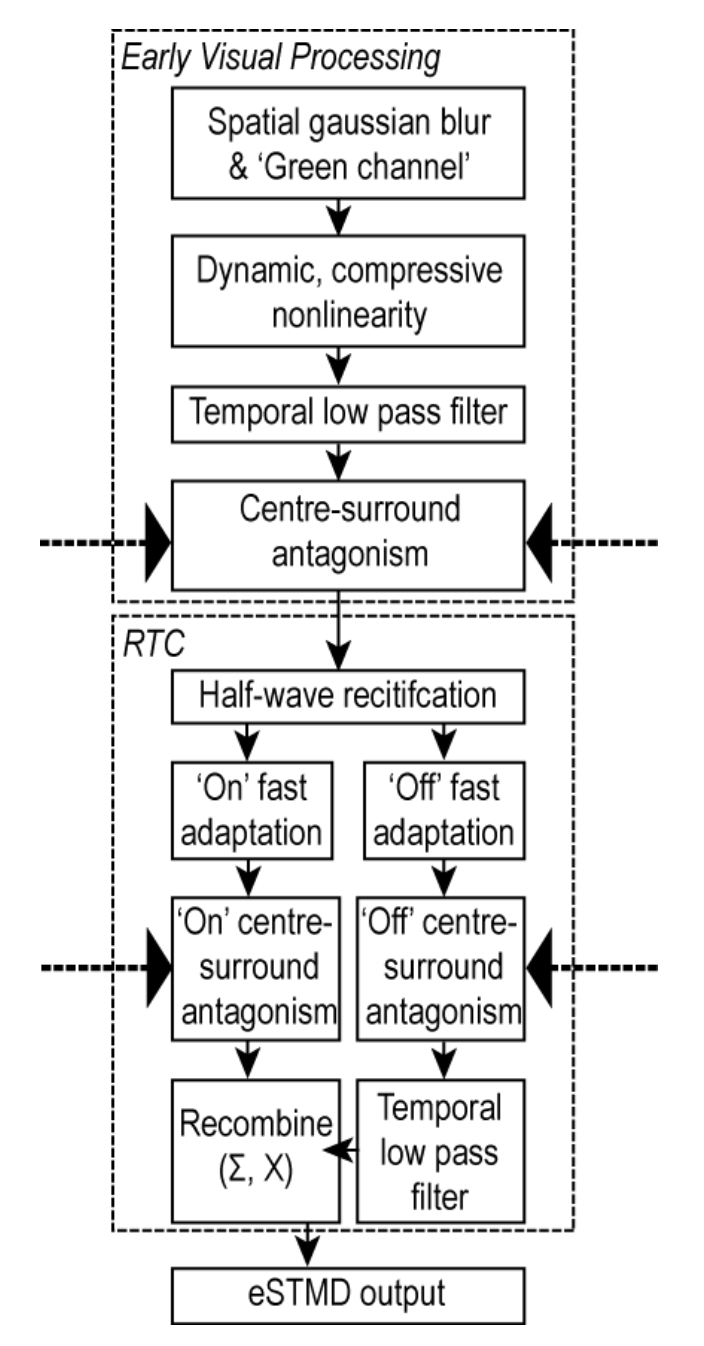
\includegraphics[scale = 0.5]{wiederman09}
\caption{CITE WIEDERMAN 2009}
\end{figure}



\end{document}
